%!TEX root = paper_main.tex
\section{Operational Lessons Learned}

While performing the Bluetana study, we learned several lessons about the
operational use of Bluetooth scanning for skimmer detection. In this section,
we provide an overview of two most important lessons we learned.

%\subsection{False positives happen, but they do not waste too much time and Few skimmers can not be detected with Bluetooth}

%\todo{finish this}

%Peterson et al.~\cite{peterson2006bluetooth} showed that 99.98\% of devices can be discovered in 6.4 s of inquiry time. This matches the observation of our measurement study, that presence of Bluetooth skimmers can be determined in a short amount of time without performing time consuming manual inspections. During the course of our study, we also saw another interesting consequence of the short time of discovery - investigators can discover presence of skimmers while simply driving by gas stations.

\subsection{Bluetooth Helps During Inspections}

Criminals hide skimmers in the crevices of gas pumps to avoid detection during inspections.
%
We witnessed several instances where investigators were unable to locate skimmers via physical inspection alone. 
%
In one incident, Bluetana flagged four devices at a station; however, no skimmers were located.
%
This result led officials more experienced in skimmer recovery to perform a second thorough inspection of the station.
%
These officials located all four skimmers.
%
The evidence provided by Bluetana forced them to continue the inspection, instead of abandoning it and leaving the devices in the field.

\begin{figure}
    \centering
    \captionsetup{justification=centering}
    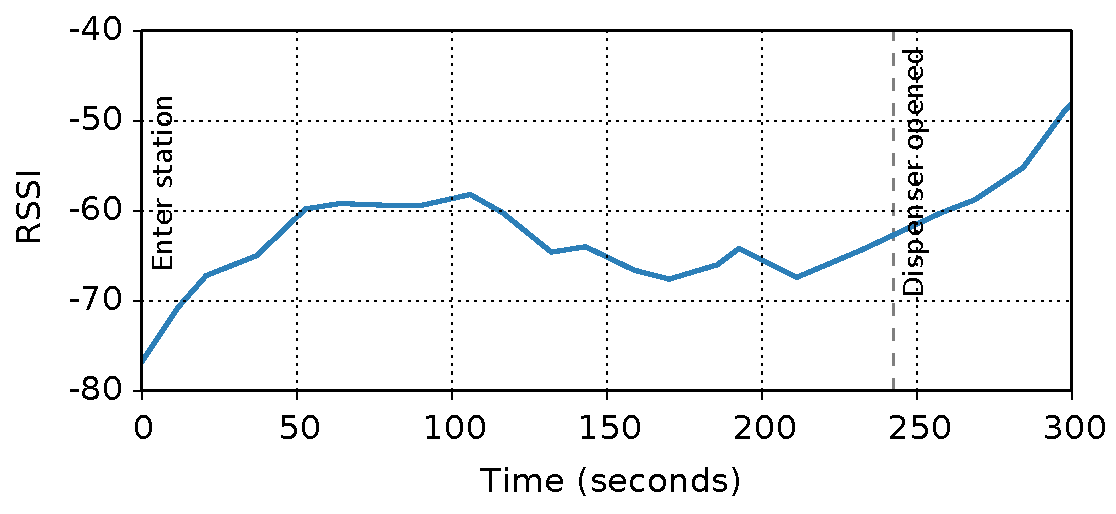
\includegraphics[width=0.6\textwidth]{skimmer/plots/rssi_jump.pdf}
    \caption{
    \label{fig:rssi_jump}
  Opening of the gas pump enclosure results in a significant jump in observed Bluetooth
  signal strength from a skimmer. 
    }
\end{figure}



Figure~\ref{fig:rssi_jump} demonstrates an instance of how the signal strength
measurements helped inspectors determine which pump had a skimmer. When the gas
pump's metal door was opened, the signal strength increased significantly,
prompting inspectors to look carefully for the skimmer in that pump.

\subsection{MAC Addresses May Indicate the Source}
\label{sec:ops:macs}

\begin{table}
\centering
\captionsetup{justification=centering}
\caption{Several geographically separated skimmers had similar MAC addresses.}
\begin{comment}
\begin{tabu} to \linewidth {lrrrrrr}
\toprule
  \textbf{Group} & \textbf{1} & \textbf{2} & \textbf{3} & \textbf{4} & \textbf{5} & \textbf{6} \\
\hline
No. of skimmers & 2 & 2 & 2 & 2 & 5 & 3 \\

Seen across stations & 1 & 1 & 2 & 2 & 2 & 2\\

Min. distance in MAC address & 17 & 166 & 9 & 3 & 4 & 4 \\

Min. distance between & & & & & & \\
closest MACs (miles) & 0 & 0 & 17 & 17 & 17 & 448 \\
\bottomrule
\end{tabu}
\end{comment}
\begin{tabu} to \linewidth {lrrrrr}
\toprule
   & \multicolumn{5}{c}{Group} \\
   \cmidrule(lr){2-6}
   & \textbf{1} & \textbf{2}  & \textbf{3} & \textbf{4} & \textbf{5} \\
\hline
Skimmers & 3 & 5 & 6 & 4 & 3 \\

Gas stations & 2 & 2 & 5 & 4 & 2\\

Min. difference in MACs & 1 & 4 & 9 & 10 & 4 \\

Closest MAC distance (in miles) & 0 & 17 & 59 & 203 & 448 \\
\bottomrule
\end{tabu}


\label{tab:mac_closeness}
\end{table}

Network equipment vendors (e.g., Bluetooth module manufacturers) tend to allocate MAC addresses sequentially by production time~\cite{wifi-macs}.
%
Therefore, if two devices have similar MAC addresses, they are likely part of the same batch of devices sold.
%
This information can be used to associate skimmer Bluetooth modules to the same board designer or crew.

We group the skimmers found by Bluetana with the same first 5 bytes of MAC address.
%
Table~\ref{tab:mac_closeness} shows five such groups.
%
We list the difference in MAC address and the geographic distance between the closest MACs in each group.
%
Skimmers in group 1 and 2 were recovered at gas stations in the same county, separated by at most 17 miles.
%
From LE sources, we know that criminals often plant skimmers across multiple stations in a given city/county, and the MAC address data collected indicates this.
%
Groups 3-5 are the most interesting, as the closest MACs in the same group are in stations across different counties.
%
The closest MACs in group 5 are at stations separated by 448 miles.
%
This may seem surprising, but LE informs us that skimmer crews avoid detection by migrating from city to city. 
